\documentclass[12pt]{amsart}
% packages
\usepackage{graphicx}
\usepackage{setspace}
\usepackage{amssymb,amsmath,amsthm,amsfonts,amscd}
\usepackage{hyperref}
\usepackage{color}
\usepackage{booktabs}
\usepackage{tabularx}
\usepackage{enumitem}
\usepackage[retainorgcmds]{IEEEtrantools}
\usepackage[notref,notcite,final]{showkeys}
\usepackage[final]{pdfpages}
\usepackage{fancyhdr}
\usepackage{upgreek}
\usepackage{multicol}
\usepackage{fontawesome}
\usepackage{halloweenmath}
% set margin as 0.75in
\usepackage[margin=0.75in]{geometry}

% tikz-related settings
\usepackage{tkz-berge}
\usetikzlibrary{calc,quotes}
\usetikzlibrary{arrows.meta}
\usetikzlibrary{positioning, automata}
\usetikzlibrary{decorations.pathreplacing}

%% For table
\usepackage{tikz}
\usetikzlibrary{tikzmark}

% theorem environments with italic font
\newtheorem{thm}{Theorem}[section]
\newtheorem*{thm*}{Theorem}
\newtheorem{lemma}[thm]{Lemma}
\newtheorem{prop}[thm]{Proposition}
\newtheorem{claim}[thm]{Claim}
\newtheorem{corollary}[thm]{Corollary}
\newtheorem{conjecture}[thm]{Conjecture}
\newtheorem{question}[thm]{Question}
\newtheorem{procedure}[thm]{Procedure}
\newtheorem{assumption}[thm]{Assumption}

% theorem environments with roman font (use lower-case version in body
% of text, e.g., \begin{example} rather than \begin{Example})
\newtheorem{Definition}[thm]{Definition}
\newenvironment{definition}
{\begin{Definition}\rm}{\end{Definition}}
\newtheorem{Example}[thm]{Example}
\newenvironment{example}
{\begin{Example}\rm}{\end{Example}}

\theoremstyle{definition}
\newtheorem{remark}[thm]{\textbf{Remark}}

% special sets
\newcommand{\A}{\mathbb{A}}
\newcommand{\C}{\mathbb{C}}
\newcommand{\F}{\mathbb{F}}
\newcommand{\N}{\mathbb{N}}
\newcommand{\Q}{\mathbb{Q}}
\newcommand{\R}{\mathbb{R}}
\newcommand{\Z}{\mathbb{Z}}
\newcommand{\cals}{\mathcal{S}}
\newcommand{\ZZ}{\mathbb{Z}_{\ge 0}}
\newcommand{\cala}{\mathcal{A}}
\newcommand{\calb}{\mathcal{B}}
\newcommand{\cald}{\mathcal{D}}
\newcommand{\calh}{\mathcal{H}}
\newcommand{\call}{\mathcal{L}}
\newcommand{\calr}{\mathcal{R}}
\newcommand{\la}{\mathbf{a}}
\newcommand{\lgl}{\mathfrak{gl}}
\newcommand{\lsl}{\mathfrak{sl}}
\newcommand{\lieg}{\mathfrak{g}}

% math operators
\DeclareMathOperator{\kernel}{\mathrm{ker}}
\DeclareMathOperator{\image}{\mathrm{im}}
\DeclareMathOperator{\rad}{\mathrm{rad}}
\DeclareMathOperator{\id}{\mathrm{id}}
\DeclareMathOperator{\hum}{[\mathrm{Hum}]}
\DeclareMathOperator{\eh}{[\mathrm{EH}]}
\DeclareMathOperator{\lcm}{\mathrm{lcm}}
\DeclareMathOperator{\Aut}{\mathrm{Aut}}
\DeclareMathOperator{\Inn}{\mathrm{Inn}}
\DeclareMathOperator{\Out}{\mathrm{Out}}
\DeclareMathOperator{\Gal}{\mathrm{Gal}}


% frequently used shorthands
\newcommand{\ra}{\rightarrow}
\newcommand{\se}{\subseteq}
\newcommand{\ip}[1]{\langle#1\rangle}
\newcommand{\dual}{^*}
\newcommand{\inverse}{^{-1}}
\newcommand{\norm}[2]{\|#1\|_{#2}}
\newcommand{\abs}[1]{\lvert #1 \rvert}
\newcommand{\Abs}[1]{\bigg| #1 \bigg|}
\newcommand\bm[1]{\begin{bmatrix}#1\end{bmatrix}}
\newcommand{\op}{\text{op}}

% nicer looking empty set
\let\oldemptyset\emptyset
\let\emptyset\varnothing

%the var phi gang
\let\oldphi\phi
\let\phi\varphi

\setlist[enumerate,1]{topsep=1em,leftmargin=1.8em, itemsep=0.5em, label=\textup{(}\arabic*\textup{)}}
\setlist[enumerate,2]{topsep=0.5em,leftmargin=3em, itemsep=0.3em}

%pagestyle
%\pagestyle{fancy} 

\begin{document}
\begin{center}
    \textsc{Math 501. HW XI\\ Ian Jorquera\\ Collaborators: Ignacio}
\end{center}
\vspace{1em}
% See http://www.mathematicalgemstones.com/maria/Math501Fall22.php
% for problems

% sage: https://sagecell.sagemath.org/
\begin{itemize}

\item[(9)] %[2+] (4 points) True or false: if every chain and every antichain of a poset P is finite, then P is finite.

Assume that every chain and anti-chain is finite.
Consider first the set of the minimal elements, call this set $S_0$. This set forms an anti chain and so must be finite. Then consider the set of elements that cover the minimal elements, call this set $S_1$. Because the elements that cover any element in a poset also form an anti-chain there must be finitely many elements covering each of the finitely many minimal elements, this means that $S_1$ is finite. Now we can inductively create the set $S_i$ which is the set of elements in the poset that covers the elements in $S_{i-1}$. Notice that this set is finite, by induction, because if $S_{i-1}$ is finite, our inductive hypothesis, then there would have the be finitely many elements covering each of the finitely many elements in $S_{i-1}$ and so $S_i$ must be finite. Furthermore because every chain is finite, there must be a largest maximal chain in the poset. Assume that the largest chain has length $k$. This would mean that $S_{j}$ is empty for any $j>k$. If it weren't then we would be able to create a chain of length $j$ going through the covers. Furthermore notice that every element in the poset is contained in at least one of these sets. Consider an element $t\in P$ and notice that either $t$ is minimal in which case it is in $S_0$ or that there is an element in $s<t$. We can repeat this with the element $s$ until we have a chain. We know that this chain would have to have length $\ell\leq k$, meaning it is contained in the set $S_{\ell}$. Finally because each $S_i$ is finite, and because there are finitely many sets, the union $\bigcup S_i$ is finite.\\



\item[(11)]  % (3-) (8 points)
% Find a finite poset P for which there is a bijection f : P \ra P such that s <= t if and only if f(s) >= f(t) (i.e., P is self-dual), but for which there is no such bijection f satisfying f(f(t)) = t for all t \in P.
In this case we need to create a poset when flipped it will also be rotated. This will force our poset to have not involutions. to make this rotation more obvious we will write the poset with the vertices a, b and c on both sides

    \begin{center}
            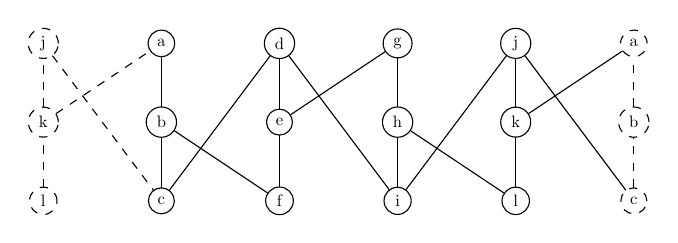
\begin{tikzpicture}
    
        % Add or remove nodes here, use the tuple for location
        \begin{scope}[every node/.style={circle,draw,scale=.6}]
        \node[style=dashed] (Am1) at (-1.5,1) {l};
        \node[style=dashed] (Bm1) at (-1.5,2) {k};
        \node[style=dashed] (Cm1) at (-1.5,3) {j};
        \node (A1) at (0,1) {c};
        \node (B1) at (0,2) {b};
        \node (C1) at (0,3) {a};
        \node (A2) at (1.5,1) {f};
        \node (B2) at (1.5,2) {e};
        \node (C2) at (1.5,3) {d};
        \node (A3) at (3,1) {i};
        \node (B3) at (3,2) {h};
        \node (C3) at (3,3) {g};
        \node (A4) at (4.5,1) {l};
        \node (B4) at (4.5,2) {k};
        \node (C4) at (4.5,3) {j};
        
        \node[style=dashed] (A11) at (6,1) {c};
        \node[style=dashed] (B11) at (6,2) {b};
        \node[style=dashed] (C11) at (6,3) {a};
    
        \end{scope}
    
        % forward(red)
        % Remove or add new edges here
        \begin{scope}[>={Stealth[black]},
                  every edge/.style={draw=black, thin}]. 
        \path [-] (Am1) edge[style=dashed] (Bm1);
        \path [-] (Bm1) edge[style=dashed] (Cm1);
        \path [-] (A1) edge[] (B1);
        \path [-] (B1) edge[] (C1);
        \path [-] (A2) edge[] (B2);
        \path [-] (B2) edge[] (C2);
        \path [-] (A3) edge[] (B3);
        \path [-] (B3) edge[] (C3);
        \path [-] (A4) edge[] (B4);
        \path [-] (B4) edge[] (C4);
        \path [-] (A11) edge[style=dashed] (B11);
        \path [-] (B11) edge[style=dashed] (C11);

        \path [-] (Bm1) edge[style=dashed] (C1);
        \path [-] (Cm1) edge[style=dashed] (A1);
        \path [-] (B1) edge[] (A2);
        \path [-] (A1) edge[] (C2);
        \path [-] (B2) edge[] (C3);
        \path [-] (C2) edge[] (A3);
        \path [-] (B3) edge[] (A4);
        \path [-] (A3) edge[] (C4);
        \path [-] (B4) edge[] (C11);
        \path [-] (C4) edge[] (A11);
        \end{scope}
    
        \end{tikzpicture}
        \end{center}

        First we will show that there is a bijection $\phi:P\ra P$ such that $s\leq t\in P$ if and only if $\phi(s)\geq \phi(t)\in P$. Such a map is $\phi(a)=f$, $\phi(b)=e$, $\phi(c)=d$, $\phi(d)=i$, $\phi(e)=h$, $\phi(f)=g$, $\phi(g)=l$, $\phi(h)=k$, $\phi(i)=j$, $\phi(j)=c$, $\phi(k)=b$, and $\phi(l)=a$. This result in the following poset

        \begin{center}
            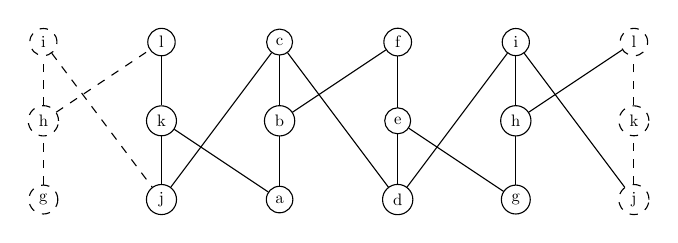
\begin{tikzpicture}
    
        % Add or remove nodes here, use the tuple for location
        \begin{scope}[every node/.style={circle,draw,scale=.6}]
        \node[style=dashed] (Am1) at (-1.5,1) {g};
        \node[style=dashed] (Bm1) at (-1.5,2) {h};
        \node[style=dashed] (Cm1) at (-1.5,3) {i};
        \node (A1) at (0,1) {j};
        \node (B1) at (0,2) {k};
        \node (C1) at (0,3) {l};
        \node (A2) at (1.5,1) {a};
        \node (B2) at (1.5,2) {b};
        \node (C2) at (1.5,3) {c};
        \node (A3) at (3,1) {d};
        \node (B3) at (3,2) {e};
        \node (C3) at (3,3) {f};
        \node (A4) at (4.5,1) {g};
        \node (B4) at (4.5,2) {h};
        \node (C4) at (4.5,3) {i};
        
        \node[style=dashed] (A11) at (6,1) {j};
        \node[style=dashed] (B11) at (6,2) {k};
        \node[style=dashed] (C11) at (6,3) {l};
    
        \end{scope}
    
        % forward(red)
        % Remove or add new edges here
        \begin{scope}[>={Stealth[black]},
                  every edge/.style={draw=black, thin}]. 
        \path [-] (Am1) edge[style=dashed] (Bm1);
        \path [-] (Bm1) edge[style=dashed] (Cm1);
        \path [-] (A1) edge[] (B1);
        \path [-] (B1) edge[] (C1);
        \path [-] (A2) edge[] (B2);
        \path [-] (B2) edge[] (C2);
        \path [-] (A3) edge[] (B3);
        \path [-] (B3) edge[] (C3);
        \path [-] (A4) edge[] (B4);
        \path [-] (B4) edge[] (C4);
        \path [-] (A11) edge[style=dashed] (B11);
        \path [-] (B11) edge[style=dashed] (C11);

        \path [-] (Bm1) edge[style=dashed] (C1);
        \path [-] (Cm1) edge[style=dashed] (A1);
        \path [-] (B1) edge[] (A2);
        \path [-] (A1) edge[] (C2);
        \path [-] (B2) edge[] (C3);
        \path [-] (C2) edge[] (A3);
        \path [-] (B3) edge[] (A4);
        \path [-] (A3) edge[] (C4);
        \path [-] (B4) edge[] (C11);
        \path [-] (C4) edge[] (A11);
        \end{scope}
    
        \end{tikzpicture}
        \end{center}

        And so $P$ is self-dual.\\
        
        Now we will show that there are no involutions that map $P$ to its dual. We will construct a bijection $\phi:P\ra P$. First we will consider the element $i$ where we know $i< h<g$ and $i<d$ and $i<j$. With $\phi$ the element $i$ can map to either $d$ or $j$.
        Case 1: $\phi(i)=j$. This would then require $\phi(h)=k$ and $\phi(g)=l$ as these are the only options that preserve the length $2$ chain $i<h<g$ as $j>k>l$. Now we will consider the element $j$. There are two options either $j$ maps to $i$ or $c$. Notice that if $\phi(j)=i$ then we would need $\phi(k)=h$ and $\phi(l)=g$ again to preserve the chain of length $2$ that is $l<k<j$. However notice that $l<h$ and $\phi(l)=g\not>k=\phi(h)$ and so it must be the case that $\varphi(j)=c$. This is enough to conclude that when $\phi(i)=j$ then $\phi$ is not an involution.\\



        Case 2: $\phi(i)=d$. This would then require $\phi(h)=e$ and $\phi(g)=f$ as these are the only options that preserve the length $2$ chain $i<h<g$ as $d>e>f$. Now we will consider the element $d$. There are two options either $d$ maps to $i$ or $c$. Notice that if $\phi(d)=i$ then we would need $\phi(e)=h$ and $\phi(f)=g$ to again preserve the chain of length $2$ that is $f<e<d$. However notice that $e<g$ and $\phi(e)=h\not>f=\phi(g)$ and so it must be the case that $\varphi(d)=c$. This is enough to conclude that when $\phi(i)=d$ then $\phi$ is not an involution.
        
\end{itemize}

\end{document}


